
\chapter{Conclusões}
\label{chap:Conclusoes}

Esta dissertação foi desenvolvida no âmbito do projeto CRIARTE, que procura integrar inteligência artificial, sensores portáteis e gémeos digitais humanos para apoiar a segurança dos trabalhadores num contexto de elevado risco, como o da construção. O trabalho analisou duas fontes de informação complementares: os sinais de ECG, frequência cardíaca e intervalos R-R recolhidos pela banda Polar H10, e as variáveis fisiológicas e comportamentais recolhidas pelo relógio Empatica EmbracePlus.

No Polar H10 foram avaliados modelos supervisionados para reproduzir um índice heurístico construído como aproximação a variações do estado fisiológico, inicialmente associado à fadiga, e as respetivas categorias. No Empatica EmbracePlus foram estudados modelos não supervisionados de agrupamento, complementados por Árvores de Decisão para permitir inferências rápidas dos agrupamentos hierárquicos. Os resultados mostram que estas abordagens são tecnicamente viáveis, mas também evidenciam a necessidade de mais dados e de validação com diferentes participantes antes de uma utilização generalizada.

\section{Resposta aos Objetivos de Investigação}
\label{sec:resposta-objetivos}

O desenvolvimento foi orientado pelo objetivo geral e pelos seis objetivos específicos apresentados no Capítulo~1. A resposta a cada objetivo é sintetizada nos pontos seguintes.

\subsection*{Objetivo geral: desenvolver e avaliar modelos para prever o estado fisiológico do trabalhador}

O objetivo geral foi concretizado através da análise de dois dispositivos e de duas estratégias de modelação. Os modelos do Polar H10 reproduziram com elevado desempenho o \textit{FatigueIndex} heurístico, enquanto os modelos aplicados ao Empatica EmbracePlus identificaram agrupamentos associados a diferentes padrões de repouso, trabalho e atividade física. Estes resultados contribuem para a construção de um módulo de análise para um gémeo digital humano, embora ainda não constituam uma validação clínica independente da fadiga, do stress, da atividade física ou de outros estados humanos.

\subsection*{Objetivo 1: analisar e caracterizar os dados fisiológicos}

Este objetivo foi cumprido através da análise dos sinais recolhidos pela banda Polar H10 e pelo relógio Empatica EmbracePlus. Foram identificadas variáveis relacionadas com ECG, frequência cardíaca, intervalos R-R, atividade eletrodérmica, movimento, sono e atividade comportamental, entre outras. A revisão do estado da arte, apresentada no Capítulo~\ref{chap:TecnologiasEmergentes}, confirmou que estas variáveis são amplamente utilizadas em estudos de monitorização fisiológica e de caracterização de estados humanos, o que apoiou a sua seleção e indicou a sua relevância para os objetivos desta investigação. A análise mostrou ainda que os dados apresentam variabilidade temporal e diferenças importantes entre participantes e atividades, fatores que influenciam diretamente o desempenho dos modelos.

\subsection*{Objetivo 2: preparar os dados para a modelação}

Este objetivo foi cumprido através da investigação, identificação e aplicação de várias etapas de preparação, incluindo tratamento de valores omissos, deteção de anomalias, normalização, escalamento, codificação de variáveis e extração de características. Estas etapas permitiram melhorar a qualidade e a comparabilidade dos dados, reduzir o impacto de imperfeições nos registos e preparar representações adequadas às diferentes abordagens de modelação. Nos dados do Empatica EmbracePlus foram ainda comparadas duas resoluções temporais: dados ao minuto e janelas de 10 minutos. Nos dados do Polar H10 foram utilizadas janelas temporais de 30 e 60 segundos, consoante a experiência. No GMM foi utilizado PCA para reduzir a dimensionalidade, enquanto o Clustering Hierárquico utilizou as 12 características originais normalizadas. A preparação dos dados foi, assim, ajustada às características de cada dispositivo, à resolução temporal analisada e aos requisitos dos modelos avaliados.

\subsection*{Objetivo 3: explorar diferentes abordagens de modelação}

Este objetivo foi explorado através de diferentes abordagens de modelação, cuja seleção foi orientada pela revisão do estado da arte apresentada no Capítulo~2. No Polar H10, foram avaliados modelos supervisionados, nomeadamente a Regressão Linear, a Regressão Logística, o SVM, o Random Forest e o XGBoost. Foram realizadas experiências com dados de um único trabalhador e com dados de vários trabalhadores, incluindo avaliações da capacidade de generalização. Foi ainda realizado um estudo de ablação, comparando a configuração completa com configurações baseadas apenas em características de ECG ou em características de HR/R-R e temporais. No relógio Empatica EmbracePlus, foram avaliados os métodos de agrupamento GMM e Clustering Hierárquico, também selecionados com base no estado da arte, com apoio de Árvores de Decisão para reproduzir as etiquetas dos agrupamentos hierárquicos.

Os resultados obtidos permitem ainda identificar uma questão relevante para a utilização futura destes modelos: o problema de \textit{cold start}. Neste contexto, as regras extraídas através das Árvores de Decisão poderão constituir uma base para definir estimativas iniciais para novos trabalhadores, utilizando perfis de referência antes de existir um volume suficiente de dados individuais. À medida que novos dados forem recolhidos, estas estimativas poderão ser progressivamente substituídas por previsões adaptadas ao perfil de cada trabalhador.

\subsection*{Objetivo 4: avaliar e comparar o comportamento dos modelos}

Este objetivo foi cumprido através da definição e aplicação de métricas, em linha com as práticas identificadas no estado da arte do Capítulo~\ref{chap:TecnologiasEmergentes}. Para os modelos supervisionados do Polar H10, foram utilizadas métricas de regressão (MSE, RMSE, MAE e $R^2$) e de classificação (Accuracy, Balanced Accuracy, Macro-F1, precisão, recall e matrizes de confusão). Na generalização entre trabalhadores através da estratégia LOSO, os modelos reproduziram as categorias do índice heurístico, embora a classe MED fosse mais difícil de distinguir das classes adjacentes. Compararam-se ainda janelas de 30 e 60 segundos no Polar H10 com dados ao minuto e janelas de 10 minutos no Empatica EmbracePlus. No relógio, os agrupamentos foram analisados através do BIC, do Silhouette Score e da variabilidade intra-cluster, enquanto as Árvores de Decisão foram avaliadas pela reprodução das respetivas etiquetas. Os dados externos permitiram avaliar os modelos num novo participante e em diferentes contextos de atividade. A aplicação conjunta destas métricas permitiu avaliar e comparar o comportamento dos modelos e identificar as abordagens mais adequadas aos dados disponíveis e aos diferentes cenários analisados. Os resultados evidenciam também a necessidade de validações adicionais com mais participantes e referências independentes.

\subsection*{Objetivo 5: selecionar uma abordagem viável para utilização em tempo real}

Este objetivo foi parcialmente cumprido, uma vez que foram exploradas abordagens com potencial para utilização em tempo real, embora ainda seja necessária validação adicional. O GMM permite realizar inferências diretamente sobre novos dados, enquanto as Árvores de Decisão podem reproduzir rapidamente as decisões do Clustering Hierárquico, que não dispõe de uma inferência direta para novas observações. Além disso, as Árvores de Decisão permitem extrair regras heurísticas simples e fáceis de implementar. Esta simplicidade pode ser particularmente relevante em contextos com um elevado fluxo de dados, nos quais decisões baseadas em regras podem permitir respostas rápidas, sem depender de processos de inferência mais complexos e reduzindo possíveis atrasos na identificação de situações de risco. No entanto, a eficácia destas abordagens e a sua capacidade de generalização ainda necessitam de uma avaliação mais aprofundada. Assim, uma abordagem híbrida, que selecione o modelo mais adequado para cada atividade ou estado, poderá ser uma solução interessante para o CRIARTE.

\subsection*{Objetivo 6: integrar o modelo num gémeo digital humano}

Este objetivo foi parcialmente cumprido. Foram definidos os principais elementos do fluxo, desde a aquisição e preparação dos dados até à inferência e à sincronização dos resultados com a representação digital do trabalhador. Contudo, à data de conclusão desta dissertação, ainda não existe no projeto CRIARTE uma estrutura totalmente montada que permita unificar todos os dados do gémeo digital, encontrando-se essa estrutura atualmente em desenvolvimento. Assim, a integração dos modelos desenvolvidos na arquitetura do gémeo digital será desenvolvida em próximas atividades do projeto CRIARTE. Os modelos avaliados e as regras heurísticas extraídas fornecem uma base para a futura implementação de um módulo de inferência orientado para a monitorização contínua; no entanto, a integração completa destes modelos num sistema operacional, incluindo o processamento contínuo dos dados e a geração automática de alertas em contexto real, não foi implementada nem validada no âmbito desta dissertação.

\section{Contribuições da Investigação}
\label{sec:contribuicoes}

As principais contribuições desta investigação são a análise conjunta de dados da banda Polar H10 e do relógio Empatica EmbracePlus; a avaliação de modelos supervisionados e não supervisionados para diferentes tipos de dados fisiológicos; o estudo de ablação das características ECG, HR e R-R; a comparação entre dados ao minuto e janelas temporais; e a utilização de Árvores de Decisão como representação rápida e interpretável dos agrupamentos hierárquicos. Foi ainda formulada uma possível abordagem híbrida de inferência para o projeto CRIARTE, combinando modelos de acordo com o seu comportamento em diferentes atividades. A metodologia e os resultados obtidos poderão servir como base e fonte de inspiração para investigadores que estudem a análise de dados fisiológicos e o treino de modelos para a previsão de estados humanos em contextos laborais, incluindo a construção, bem como para a sua adaptação a outros contextos.

No âmbito da disseminação científica, foi elaborado o artigo de revisão sistematizada intitulado ``\textit{A Review of Physiological Monitoring and Prediction in Workers in High-Risk Construction Environments}''~\cite{freitas2026physiological}, baseado no estado da arte desenvolvido nesta investigação. O artigo foi aceite e apresentado na conferência \textbf{INISTA 2026}~\cite{inista2026} pelo autor desta dissertação, a 17 de setembro de 2026, em Guimarães, Portugal, constituindo uma contribuição para a divulgação dos fundamentos e resultados da investigação. Após a conferência, está prevista a sua inclusão nas atas e a disponibilização através da \textbf{IEEE Xplore}~\cite{ieeexplore}, biblioteca digital especializada em publicações científicas e técnicas. Esta apresentação é documentada na Figura~\ref{fig:inista2026}.

\begin{figure}[H]
\centering
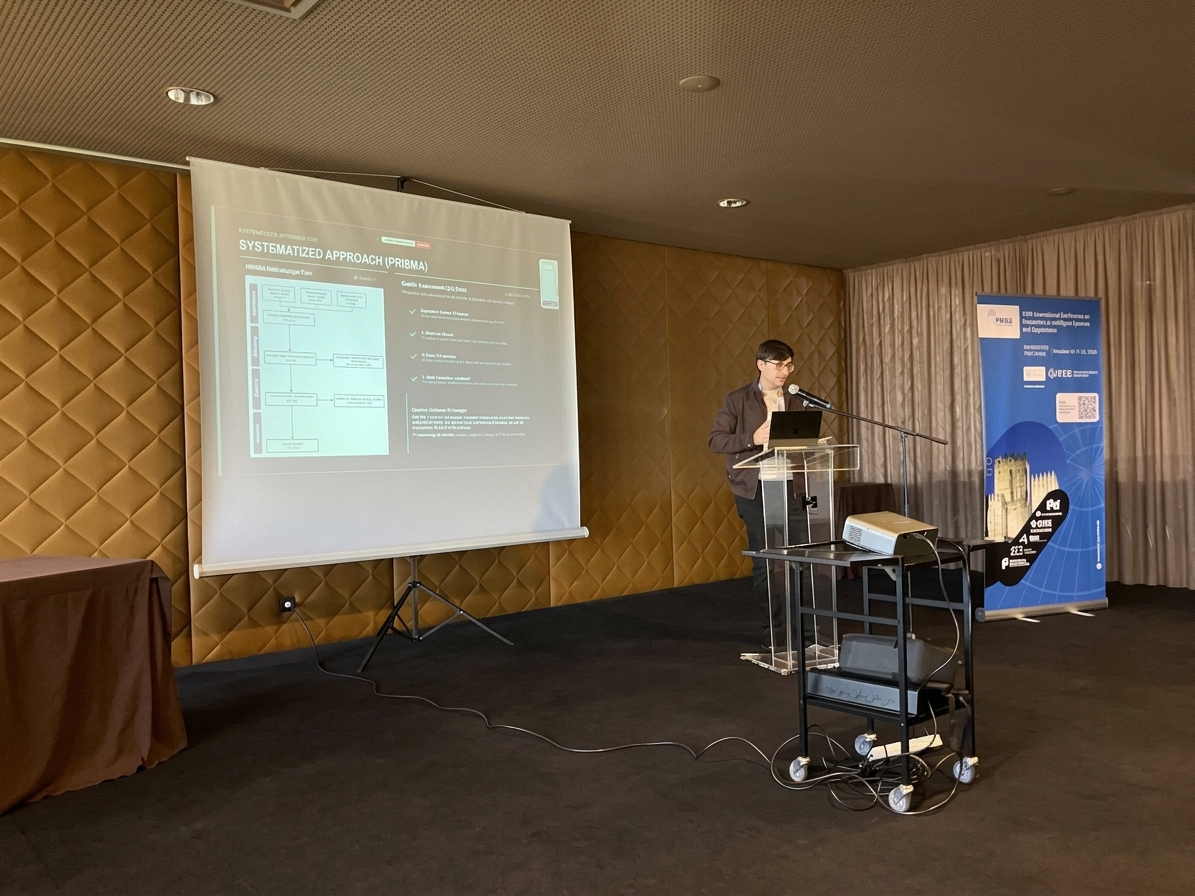
\includegraphics[width=0.6\textwidth]{ch5/assets/inista2026.jpg}
\caption{Apresentação do artigo na conferência INISTA 2026, Guimarães, Portugal, 17 set 2026.}
\label{fig:inista2026}
\end{figure}

Foi também submetido à revista \textbf{Advanced Engineering Informatics}~\cite{advancedengineeringinformatics}, publicada pela editora Elsevier, o artigo ``\textit{Unsupervised Physiological State Clustering for Construction Worker Fatigue Monitoring: Comparing GMM and Hierarchical Clustering Across Temporal Resolutions}''. Este trabalho reúne os resultados da análise dos dados do relógio Empatica EmbracePlus, incluindo o GMM, o Clustering Hierárquico, as Árvores de Decisão e a avaliação com dados externos. No momento de redação desta dissertação, o artigo encontra-se em revisão por pares. Ainda não foi tomada qualquer decisão editorial quanto à sua aceitação ou rejeição, pelo que a submissão é apresentada apenas como uma contribuição potencial para a disseminação científica dos resultados obtidos.

\section{Limitações Identificadas}
\label{sec:limitacoes}

Apesar dos resultados encorajadores, o trabalho desenvolvido apresenta algumas limitações relevantes, que devem ser consideradas na interpretação dos resultados e no planeamento de desenvolvimentos futuros:

\begin{itemize}
\item \textbf{Natureza heurística do FatigueIndex:} 
Uma limitação importante da metodologia está relacionada com a natureza heurística do \textit{FatigueIndex} e com a ausência de etiquetas fisiológicas independentes para validação. O índice constitui uma representação quantitativa construída a partir de características fisiológicas, não correspondendo a uma medida clínica direta de fadiga, stress ou de outros estados psicofisiológicos. Assim, os resultados obtidos representam a capacidade dos modelos para estimar esta representação, não permitindo estabelecer, por si só, uma avaliação clínica desses estados sem validação adicional.

\item \textbf{Dados em falta no Polar H10:} 
Uma limitação importante está relacionada com a quantidade significativa de dados em falta nos registos da banda Polar H10 de alguns trabalhadores, sobretudo nas variáveis de frequência cardíaca (HR) e nos intervalos RR. Esta perda pode estar associada a medições incorretas, ao movimento do trabalhador, às condições do contexto de obra, a problemas de calibração ou a falhas de ligação entre o dispositivo e o sistema de registo. O conforto e a interação natural do trabalhador também podem influenciar a recolha, uma vez que a transpiração, a irritação ou alterações na posição da cinta podem modificar o contacto com a pele e provocar valores em falta ou artefactos nos sinais. Estes efeitos podem ser confundidos pelos modelos com alterações fisiológicas reais, condicionando as características obtidas e os resultados. Embora os modelos tenham apresentado desempenho satisfatório e capacidade de generalização para trabalhadores não observados durante o treino, não é possível excluir a influência destas limitações. Este tipo de ruído é expectável em recolhas reais, pelo que os modelos devem ser preparados para lidar com estas imperfeições ou minimizar o seu impacto.

\item \textbf{Restrições da recolha de dados:} 
Existiram algumas restrições associadas ao próprio projeto que condicionaram a recolha de dados. A utilização de um único relógio Empatica EmbracePlus limitou a possibilidade de recolher dados de vários trabalhadores em simultâneo durante as simulações. Além disso, o acesso ao ecossistema do dispositivo, incluindo a aplicação e a plataforma de gestão dos dados, envolve custos de licenciamento, o que dificultou a disponibilização de um maior número de equipamentos. A escolha deste dispositivo foi, contudo, justificada pela qualidade, robustez e fiabilidade dos dados recolhidos, pela sua menor suscetibilidade ao ruído e pelo reconhecimento destas características na literatura e na prática. A preparação dos cenários simulados e a compensação dos trabalhadores envolvidos limitaram também a realização de um maior número de experiências com ambos os dispositivos. Estas condições podem ter reduzido a diversidade dos dados disponíveis para o treino e dificultado a avaliação da capacidade de generalização dos modelos para trabalhadores não observados. Assim, será necessária uma recolha mais ampla e diversificada para confirmar estes resultados e melhorar o desempenho dos modelos.

\item \textbf{Ausência de etiquetas independentes:} 
Outra limitação importante está relacionada com a ausência de etiquetas independentes para validar os estados psicofisiológicos analisados. Os agrupamentos obtidos foram interpretados com base nas características dos dados de cada \textit{cluster} e na sua distribuição temporal, procurando identificar os possíveis estados representados. Embora esta análise tenha procurado ser objetiva e baseada nos padrões observados nos dados, a ausência de avaliações subjetivas ou fisiológicas recolhidas simultaneamente com os dados do Empatica EmbracePlus limita a validação independente destas interpretações. Assim, apesar de os agrupamentos poderem representar adequadamente os padrões presentes nos dados, existe a possibilidade de erros na interpretação dos estados a eles associados, sendo necessária uma validação adicional para confirmar estas interpretações.
\end{itemize}

\section{Trabalho Futuro}
\label{sec:trabalho-futuro}

Para superar estas limitações e aproximar o sistema de uma aplicação real, propõem-se as seguintes linhas de investigação:

\begin{itemize}
\item \textbf{Melhoria da recolha de dados:} 
Como trabalho futuro, será necessário recolher dados de mais participantes e em diferentes atividades, aumentar o número de dispositivos disponíveis e repetir as experiências em condições mais variadas. Deverão também ser reforçados os procedimentos de calibração, verificação da ligação e controlo de qualidade dos sinais, bem como definidos protocolos de colocação e utilização dos dispositivos adequados ao contexto de obra. Estas medidas poderão reduzir a perda de dados e permitir distinguir mais claramente os problemas de medição, movimento, ligação e recolha das variações fisiológicas reais.

\item \textbf{Etiquetas e modelos:} 
Uma abordagem a testar consiste na recolha de autorrelatos dos trabalhadores durante a realização das atividades, através de níveis ou escalas definidos para avaliar estados psicofisiológicos relevantes. Estes relatos poderiam ser associados temporalmente às janelas dos sinais recolhidos pelos dispositivos, permitindo criar etiquetas baseadas na perceção dos próprios trabalhadores e treinar modelos supervisionados de \textit{Machine Learning} e \textit{Deep Learning}. Esta estratégia poderá reduzir a necessidade de construir índices heurísticos ou de definir os alvos exclusivamente através de métodos de agrupamento. Poderiam ainda ser avaliadas arquiteturas LSTM, Bi-LSTM e 1D-CNN, bem como outras arquiteturas identificadas no estado da arte que não foram testadas nesta investigação, desde que a quantidade de dados e os recursos computacionais disponíveis permitam controlar o risco de sobreajuste.

\item \textbf{Distinção entre estados físicos e mentais:} 
Embora esta investigação tenha procurado caracterizar diferentes estados humanos, incluindo fadiga física e mental, stress e carga de trabalho, os resultados obtidos apontaram sobretudo para níveis de atividade física e esforço. No caso do Polar H10, os resultados permitiram caracterizar principalmente níveis relativos de atividade física e esforço. No caso do Empatica EmbracePlus, os agrupamentos identificados permitiram reconhecer diferentes estados físicos e contextuais, incluindo períodos associados ao trabalho e a possíveis situações de esforço cognitivo, mas não permitiram caracterizar de forma específica estados mentais. Como desenvolvimento futuro, poderá ser estudado um conjunto de modelos orientado especificamente para estados mentais, como fadiga mental, stress e carga de trabalho cognitiva, explorando diferentes abordagens de aprendizagem e diferentes formas de caracterizar estes estados.

\item \textbf{Integração no gémeo digital:} 
Com base nos resultados obtidos e nos modelos treinados, poderá também avançar-se para o desenho de uma arquitetura de integração no gémeo digital do projeto CRIARTE. Esta arquitetura deverá estudar a integração dos modelos e das suas inferências no ecossistema baseado em ROS2 utilizado pelo projeto, permitindo partilhar os dados dos sensores, as previsões e os alertas com os restantes componentes do gémeo digital. Poderá ainda ser considerada uma solução distribuída, na qual as inferências mais rápidas e a geração de alarmes sejam realizadas localmente, através de aplicações em dispositivos de \textit{edge} presentes na obra, enquanto os modelos mais pesados e as análises que não exigem resposta imediata sejam executados através de \textit{cloud computing}. A comparação destas alternativas deverá considerar a latência, a conectividade, os recursos computacionais, o consumo energético, a privacidade dos dados e a fiabilidade dos alertas.

\item \textbf{Validação do FatigueIndex:} 
Será igualmente importante realizar uma validação independente do \textit{FatigueIndex}, recolhendo simultaneamente os dados do Polar H10 e avaliações validadas de fadiga e stress, complementadas, quando adequado, por avaliações de profissionais de saúde e testes de desempenho ou atenção. O \textit{FatigueIndex} não deve ser interpretado como uma medida direta destes estados, uma vez que os resultados deste trabalho sugerem que representa sobretudo níveis relativos de atividade física, esforço e estado fisiológico. A comparação com referências externas permitirá avaliar a sua relação com a fadiga e o stress e verificar o significado das categorias LOW, MED e HIGH. Deverá também ser avaliado o efeito de diferentes pontos de corte na conversão do índice contínuo em categorias, uma vez que outras estratégias além dos percentis P33 e P66 podem produzir categorias com significado diferente e influenciar o desempenho dos modelos. Este tipo de estudo deverá ser realizado com aprovação ética e acompanhamento especializado.
\end{itemize}

\section{Reflexões Finais}
\label{sec:reflexoes-finais}

Esta dissertação reuniu esforços de investigação e desenvolvimento centrados na análise de dados fisiológicos recolhidos por dispositivos portáteis e na aplicação de modelos de inteligência artificial à segurança laboral. A utilização conjunta do Polar H10 e do Empatica EmbracePlus permitiu explorar duas estratégias complementares: a aprendizagem supervisionada para reproduzir o \textit{FatigueIndex} e a aprendizagem não supervisionada para identificar agrupamentos associados a diferentes padrões de atividade e contexto. Os resultados mostram que estas abordagens podem contribuir para caracterizar o estado fisiológico do trabalhador e constituem uma base experimental relevante para o desenvolvimento do projeto CRIARTE.

O trabalho permitiu também evidenciar alguns dos desafios associados à aplicação destes sistemas em contextos reais. A qualidade e a disponibilidade dos sinais, a variabilidade entre trabalhadores, a ausência de etiquetas independentes e a dificuldade em distinguir atividade física de estados mentais limitam a interpretação dos resultados. Por isso, os modelos desenvolvidos não devem ser entendidos como instrumentos clínicos ou como substitutos da avaliação humana, mas como componentes de apoio à monitorização e à tomada de decisão, sujeitos a validação adicional e supervisão adequada.

A continuação deste trabalho deverá combinar uma recolha de dados mais ampla, avaliações reportadas diretamente pelos trabalhadores e modelos capazes de representar diferentes estados físicos e psicofisiológicos. A integração das inferências no ecossistema ROS2 do CRIARTE, complementada por arquiteturas de processamento local e em cloud, poderá aproximar os resultados experimentais de uma aplicação operacional. Neste contexto, o gémeo digital humano deverá ser concebido como uma ferramenta complementar, orientada para a prevenção e para o apoio à segurança, capaz de ampliar a capacidade de acompanhamento do trabalhador sem substituir o conhecimento, a responsabilidade e a decisão humanas.